\chapter{Dark Energy and Modified Gravity}
\label{chpt:de_mg}
In this chapter we briefly introduce how we can modify Einstein`s general relativity, what are reasons for such modifications, and main ideas behind adding new degrees of freedom to the Einstein equations. We describe one particular model of modified gravity in more detail -- the $f(R)$ theory and chameleon gravity.

%%%%%%%%%%%%%%%%%%%%%%%
% Standard LCDM model
%%%%%%%%%%%%%%%%%%%%%%%
\section{Standard \LCDM\ model -- successes and issues}
Standard cosmological model, the \LCDM\ model or the concordance model, assumes that the Universe was created in the Big Bang from infinitely hot and dense energy and now is the Universe composed of about 5\% ordinary matter, 27\% dark matter, and 68\% dark energy \parencite{redefineLCDM}. The \LCDM\ model is based upon two theoretical models -- the Standard Model of Particle Physics and  the General Theory of Relativity. The model also assumes that the universe is homogeneous and isotropic on sufficiently large (cosmic) scales. The model is mathematically described above in \autoref{chpt:cosmo_evol}.

The \LCDM\ model represents general relativity with a cosmological constant \(\Lambda\) which is associated with dark energy and a universe containing sufficiently massive dark matter particles, i.e., cold dark matter. However, the nature of both dark energy and dark matter is unknown.

In 1948, \textcite{PhysRev.74.505.2} suggested that the elements could have been made during the early hot matter-energy phase associated with the Big Bang and predicted their representation -- hydrogen about 75\%, helium about 25\% and small amounts of deuterium, lithium, and other light elements.

The other great success of the Big bang model is prediction of the Cosmic Microwave Background (CMB) radiation and its temperature. In 1948, \textcite{1948Natur.162..774A} calculated the present temperature of the CMB to be about 5 K, remarkably close to the modern value of about 2.73 K, determined by the COBE satellite. In addition, the COBE results showed an extremely isotropic and homogeneous CMB. This led to the need for an inflationary phase \parencite{1981PhRvD..23..347G} of strongly accelerated expansion prior to the decoupling of photons from ordinary matter.

The \LCDM\ model has an additional major assumption about existence of dark matter. The notion of dark matter arose from observations of large astronomical objects such as galaxies and clusters of galaxies, which displayed gravitational effects that could not be accounted for by the visible matter. In particular, the observations of \textcite{1980ApJ...238..471R}, who measured the rotation curves for the luminous matter of many spiral galaxies together with the observations of \textcite{1978PhDT.......195B}, who compiled 21 cm rotation curves for neutral hydrogen gas that extended far beyond the luminous matter of each galaxy, showed that the composite rotation curves were essentially flat out to the edge of the 21 cm data. This implied that considerably more mass was required to be present in each galaxy. This invisible matter was called dark matter and since to date no dark matter has been definitely detected and the nature of dark matter remains unknown.

The notion of dark energy arose from two sets of observations of supernovae of Type Ia by \textcite{riess} and \textcite{1999ApJ...517..565P} that suggested that the expansion of the universe is accelerating. The conclusion from these observations was that the universe had to contain enough energy to overcome gravity. This energy was named “dark energy.”

\subsection{Cosmological constant problem}
\label{ssec:lambda}
Standard cosmological \LCDM\ model described above is in a good agreement with all measurements of CMB \parencite{planck_cosm}, type Ia supernovae \parencite{Abbott_2019}, or BAO \parencite{BAO_results}. However, this concordance model, and namely the cosmological constant, has some significant fundamental problems. Usually, the fine-tuning of the cosmological constant is presented as the main issue but the real issue with the cosmological constant is radiative instability, and the need to \textbf{repeatedly} fine tune whenever the higher loop corrections are included. We will describe here only the main idea behind these problems, for more detailed overview see e.g. \textcite{2015arXiv150205296P,2012CRPhy..13..566M}.

The action of the general relativity, together with the action describing matter, is
\eq{
	\label{eq:S_GR}
	S=\frac{\Mpl^2}{2}\int\dd^4x\dg\left(R-2\Lambda_B\right)+S_m[\psi_m;g_\uv]\,,
}
where $\Mpl\equiv(\sqrt{8\pi G})^{-1}$ is the reduced Planck mass, $R$ is the Ricci scalar (curvature), $\Lambda_B$ the bare cosmological constant and $S_m[\psi_m;g_\uv]$ represents the action of matter fields. The first term $(R)$ is the standard Einstein-Hilbert action. The \textit{bare} cosmological constant appears in the second term of the above expression and it is merely a new parameter of the total action. As it is compatible with general covariance this term appears to be totally natural from the relativistic point of view. The third term in the above equation denotes the generic matter action. Variation of the total action with respect to the metric tensor leads to the Einstein equations of motion
\eq{
    R_\uv-\frac12Rg_\uv+\Lambda_Bg_\uv=\frac{1}{\Mpl^2}T_\uv\,,
}
where the stress-energy tensor is defined by
\eq{
    T_\uv=-\frac{2}{\dg}\frac{\delta S_m}{\delta g^\uv}\,.
}
As shown by \textcite{1968SPhD...12.1040S}, when one takes into an account quantum field theory the picture is changed. The stress energy tensor of a field placed in the vacuum state is given by
\eq{
    \left\langle0\left|T_\uv\right|0\right\rangle=-\rho\vac g_\uv\,,
}
where $\rho\vac$ is the constant energy density of the vacuum. The vacuum fluctuations are just a specific type of energy and, in general relativity, all forms of energy gravitate. Therefore, the Einstein equations when quantum field theory is taken into account are
\eq{
    R_\uv-\frac12Rg_\uv+\Lambda\eff g_\uv=\frac{1}{\Mpl^2}T_\uv\,,
}
where
\eq{
    \Lambda\eff=\Lambda_B+\frac{1}{\Mpl^2}\rho\vac\,.
}
Therefore, we conclude that the effective cosmological constant is the sum of the bare cosmological constant and of a contribution originating from the vacuum fluctuations. The effective cosmological constant $\Lambda\eff$ is the quantity that one can observe and constrain when tests of the Einstein equations are carried out. The problem is that $\rho\vac$ is made of several terms which are all huge in comparison with the observed value of $\Lambda\eff$ and need to be fine-tunned.
\subsubsection{Phase Transitions}
\begin{sloppypar}
Another problem with fine-tuning of the cosmological constant comes from changes in the vacuum energy during phase transitions such as was the electro-weak phase transition. The contribution to the vacuum energy coming from the minimum of a potential of some field, in this case the Higgs field, changes as the field takes its new position after the transition. One can calculate this contribution \parencite{2012CRPhy..13..566M} and for the the mass of the Higgs boson $m_H=125$ GeV arrives at
\end{sloppypar}
\eq{
    \rho\vac^{EW}\simeq -10^{55}\rho\crit\,.
}
For the quantum chromo-dynamics transition, one can compute
\eq{
    \rho\vac^{EW}\simeq10^{45}\rho\crit\,.
}
If we fine-tune the vacuum energy to be zero today it had to be non-zero (and huge) before each of these transitions.
\subsubsection{Zero-Point Energy Density}
When we consider a simple real free scalar field with the potential $V(\Phi)=2m^2\Phi^2/2)$ we will arrive at the vacuum energy
\eq{
    \left\langle \rho \right\rangle = \left\langle0\left|T_{00}\right|0\right\rangle=\frac{1}{2\pi^3}\frac12\int\dd^3k\sqrt{k^2+m^2}\,.
}
This contribution to the cosmological constant blows up in the ultra-violet regime and is infinite. But this is nothing new in the quantum field theory. If we apply the dimensional regularization \parencite{tHooft:1972tcz} and subtract the pole as usual, one is left with finite energy density of the vacuum
\eq{
    \left\langle \rho \right\rangle = \frac{m^4}{64\pi^2}\ln{\left(\frac{m^2}{\mu^2}\right)}\,,
}
where $\mu$ is a regularization scale. We see that the contribution is proportional to the fourth power of the mass of the particle and therefore, e.g., the photon does not contribute to the vacuum energy density. The equation was derived for free scalar field but similar contributions with different pre-factors can be computed for all other fields. The overal vacuum energy density is then
\eq{
    \label{eq:vac_all}
    \rho\vac=\sum_in_i\frac{m_i^4}{64\pi^4}\ln{\left(\frac{m_i^2}{\mu^2}\right)} + \rho_B + \rho\vac^{EW} + \rho\vac^{QCD}\,,
}
where $n_H=1$ for the Higgs boson, $n_f=4$ for fermions and $n_V=3$ for massive vector fields. For the renormalization scale $\mu\simeq3\times10^{-25}$, as discussed in \textcite{2011arXiv1105.6296K}, one calculates the contribution from the zero-point energy of particles to be  $\rho\vac\simeq-2\times10^8$ GeV$^4$
\subsubsection{Radiative instability}
The one loop contributions \eqref{eq:vac_all} to the vacuum energy can be fine-tunned via the bare cosmological constant and associated $\rho_B$. Even though the cancellation has to be very precise (one part in $\sim10^{60}$) we can be fine with this solution. Problems come with two-loops correction which is not significantly suppressed with respect to the one loop contribution \todo{CITE}. Therefore, the cancellation imposed at one loop is completely spoilt, and one must retune the finite contributions in the counterterm to more or less the same degree of accuracy. If we go further, to the three loops, four loops, and so on, we are required to fine tune each time to an extreme accuracy. This is radiative instability and main cosmological constant problem.



%%%%%%%%%%%%%%%%%%%%%%%
% f(R)-gravity
%%%%%%%%%%%%%%%%%%%%%%%
\section{$f(R)$-gravity}
One of~the~simplest modified gravity models is the~so-called $f(R)$ gravity in~which we consider general functions of~the~Ricci scalar $R$ in~the~action
\eq{
	\label{eq:S_fr}
	S=\frac{\Mpl^2}{2}\int\dd^4x\dg\left[F(R)\right]+S_m[\psi_m;g_\uv]\,,
}
where $F(R)=R+f(R)$ and~$S_m$ is the~matter action with~matter fields $\psi_m$ which are minimally coupled to~gravity, i.e. they interact with~gravity only through the~determinant of~the~metric $\dg$ and~the~canonical kinetic term $-\frac12g^\uv\partial_\mu\psi\partial_\nu\psi$. The~matter fields $\psi_m$ obey standard conservation equations and~therefore the~metric $g_\uv$ corresponds to~the~Jordan frame.

Variation with~respect to~the~metric $g^\uv$ gives us the~equation of~motion
\eq{
	\label{eq:fR}
	F\R R_\uv-\frac{1}{2}F g_\uv+g_\uv\Box F\R-\nabla_\mu\nabla_\nu F\R=\frac{1}{\Mpl^2}T_\uv\,.
}
For~$f(R)=-2\Lambda$ the~standard Einstein gravity is reconstructed. Taking the~trace of~\eqref{eq:fR} we get
\eq{
	\label{eq:fR_tr}
	3\Box F\R+F\R R-2F=\frac{1}{\Mpl^2}T\,.
}
We see that there is a~propagating scalar degree of~freedom, so-called \textit{scalaron} $F\R$ with~mass $m^2=F\R/(3F\RR)$, which corresponds to~the~scalar field conformally coupled to~matter in~the~Einstein frame.

To~get the~inflation we need a~solution that approaches the~de Sitter solution characterized by vacuum space with~constant positive curvature. Thus $\Box F\R=0$ and~\eqref{eq:fR_tr} becomes
\eq{
	F\R R-2F=0.
}
For~example, the~model $F(R)=\alpha R^2$ gives rise to~an~asymptotically exact de Sitter solution and~can be responsible for~the~inflation in~the~early Universe. In~the~model $f(R) = R + \alpha R^2$, the~inflation ends when the~quadratic term becomes smaller than the~linear term. As at~the~present epoch is the~curvature very small this model is not suitable to~realize the~present cosmic acceleration. Models like $f(R)=-\alpha/R^n$ with~$\alpha>0,\ n>0$ could in~principle give rise to~the~present acceleration. However, these models do not satisfy local gravity constraints because of~the~instability associated with~negative values of~$f\RR$. Moreover, the~standard matter epoch is not present because of~a~large coupling between the~Ricci scalar and~the~non-relativistic matter.

There are four conditions for~the~viability of~\fR\ models \parencite{Amendola_2007}
\begin{itemize}
	\item $F\R>0\ (\rm{for\ } R>R_0)$, where $R_0$ is the~Ricci scalar at~the~present epoch,\\
	-- required to~avoid anti-gravity \parencite{2010deto.book.....A}\\
	\item $F\RR>0\ (\rm{for\ } R>R_0)$,\\
	-- required for~consistency with~local gravity tests \parencite{2005gr.qc.....5136O}, for~the~presence of~the~matter-dominated epoch \parencite{2007PhRvL..98m1302A} and~the~stability of~cosmological perturbations \parencite{2007PhRvD..75d4004S}\\
	\item $F(R)\rightarrow R-2\Lambda\ (\rm{for\ } R\gg R_0)$,\\
	-- required for~consistency with~local gravity tests \parencite{2008PhRvD..77b3507T} and~for~the~presence of~the~matter-dominated epoch \parencite{Amendola_2007}\\
	\item $0<\frac{RF\RR}{F\R}<1\ (\rm{for\ } F\R R-2F=0)$.\\
	-- required for~the~stability of~the~late-time de Sitter solution \parencite{1988PhLB..202..198M}
\end{itemize}
Some examples of~\fR\ models that satisfy these conditions:
\eq{
	f(R)&=-\mu R_c(R/R_c)^p	&\mbox{for\ }&0<p<1;\ \mu,R_c>0\,,\\
	f(R)&=-\mu R_c\frac{(R/R_c)^{2n}}{(R/R_c)^{2n}+1} 	&\mbox{for\ }&n,\mu,R_c>0\,,\\
	f(R)&=-\mu R_c\left[1-(1+R^2/R^2_c)^{-n}\right] 	&\mbox{for\ }&n,\mu,R_c>0\,,\\
	f(R)&=-\mu R_c\tanh(R/R_c)	&\mbox{for\ }&\mu,R_c>0\,.
}
One of~the~main predictions of~\fR\ gravity is a~different structure formation history than in~\LCDM. For~the~large-scale structure formation on~subhorizon scales \mbox{$k\gg H$} in~quasi-static approximation one gets the~modified equation for~matter density perturbation \parencite{2011RSPTA.369.4947B}
\eq{
	\ddot{\delta}_m+2H\dot{\delta}_m-4\pi G\eff \rho_m\delta_m\approx0\,,
}
where the~effective gravitational constant is defined by
\eq{
	G\eff \equiv\frac{G}{1+f\R}\frac{4k^2+3a^2m^2}{3k^2+3a^2m^2}\,.
}
On~scales much larger than the~scalaron Compton wavelength $m\mins$, gravity is unmodified aside from the~overall reduction factor $f\R$. However, on~smaller scales the~gravitational coupling increases by the~factor $4/3$. As the~scalaron mass $m$ and~the~factor $f\R$ depend on~curvature (local density), the~chameleon mechanism discussed earlier can prevent the~detection of~this effect in~the~Solar System.

%%%%%%%%%%%%%%%%%%%%%%%%%%%%%%
% Jordan vs. Einstein Frame
%%%%%%%%%%%%%%%%%%%%%%%%%%%%%%
\subsection{Jordan vs. Einstein Frame}
The~action \eqref{eq:S_fr} is described in~the~so-called Jordan frame, where the~matter fields are minimally coupled to~the~metric and~follow geodesics. We can also describe the~action in~the~so-called Einstein frame, where ``standard'' gravity is restored. Using the~conformal transformations
\eq{
\label{eins_trans}
\begin{split}
\tilde{g}_\uv &\equiv F\R g_\uv \,, \\
\phi &\equiv\Mpl\sqrt\frac32\ln F\R \,, \\
A(\phi) &\equiv F\R^{-1/2}\,, \\
V(\phi) &\equiv\frac{\Mpl^2}{2} \frac{F\R R - F}{F\R^2}\,,
\end{split}
}
we can rewrite the~action \eqref{eq:S_fr}
\eq{
\label{eq:S_ein_fr}
S=\int\dd^4x\dgt\left[\frac{\Mpl^2}{2}\tilde{R} - \frac12(\partial\phi)^2-V(\phi)\right]+S_m[\psi_m;A^2(\phi)\tilde{g}_\uv],
}
where tildes denote quantities in~the~Einstein frame. This action looks like the~Einstein-Hilbert action with~minimally coupled scalar but now the~matter fields are also coupled with~the~scalar field via factor $A(\phi)$. %Also from the~second row of~\eqref{eins_trans} can be seen why is the~Brans-Dicke parameter restricted to~be $\omega>-3/2$.

There is a~difference between whether one takes action \eqref{eq:S_fr} or \eqref{eq:S_ein_fr} to~be the~fundamental action defining the~modified gravity. In~the~former one, there is only one coupling constant $\beta$, defined by $A(\phi)=\exp(\beta\phi/\Mpl)$, for~all matter fields. If one takes the~action in~the~Einstein frame to~be the~fundamental one the~matter action is replaced by $S_m[\psi_m;A^2(\phi)\tilde{g}_\uv]\rightarrow S_i[\psi_i;A_i^2(\phi)\tilde{g}_\uv]$ where one can define the~coupling strengths $\beta_i$ to~the~different matter components to~be different. This is very important for~tests of~modified gravity. For~instance, if there is minimal coupling to~the~baryonic matter, $\beta_b=0$, Solar System or astrophysical tests do not constraint coupling strength to~the~cold matter $\beta_c$ whereas the~cosmological observations do.

Note that the~coupling constant for~\fR\ is $\beta=\sqrt{1/6}$ but for~other more general theories this coupling can vary. Even for~\fR\ theories, one expects that loop corrections can change the~coupling strength. Also, other theories such as the~Jordan--Brans--Dicke theory, Kaluza--Klein theories, and~higher derivative theories of~gravity, can be formulated in~two different ways \parencite{Faraoni:1998qx}.

These two conformally related frames are physically equivalent, i.e. physical observations are frame independent, but the~frame dependence of~cosmological perturbations has led to~confusion in~the~past. There have been many debates about the~(in)equivalence of~these frames \parencite{Postma:2014vaa} and~whether which one is the~physical \parencite{Faraoni:1999hp}. Many contradictory arguments (sometimes incorrect) of~both sides result in~confusion and~ambiguous viewpoints.

It has been shown in~\textcite{Magnano:1993bd} that these two frames are \textit{mathematically} equivalent, i.e. every solution in~one frame implies an~existence of~a~solution in~the~other frame and~can be mapped into this frame. The~confusion about their physical equivalence comes from interpretations of~experiment results. For~example, \textit{ordinary} cosmology described by Einstein’s theory leads to~an~expanding universe solution. Coming to~the~Jordan frame we can interpret the~scale factor as a~scalar field which is coupled to~matter. In~this case, the~redshift of~spectral lines is no longer interpreted as an~effect due to~the~expansion of~the~Universe, but due to~growth of~coupling constants such that the~present transition energies are higher than those in~the~past. Hence the~Jordan frame physicist does not see an~expanding Universe, but growing coupling constants. Nevertheless, the~measured redshift of~spectral lines is the~same for~both frames.

Both frames have some issues with~fundamental principles. In~the~Jordan frame, the~weak energy condition can be violated and~hence states with~the~negative energy are possible. Moreover, there is no guarantee of~stability of~the~ground state. All \textit{classical} fields are believed to~satisfy the~energy condition but no so in~quantum theories. On~the~other hand in~the~Einstein frame, the~weak energy condition is satisfied but due to~the~non-universal coupling of~the~matter fields, the~equivalence principle is violated. However, this violation is only weak and~can pass the~Solar system tests.

%%%%%%%%%%%%%%%%%%%%%%%%%%%%%%
% Screening Mechanisms
%%%%%%%%%%%%%%%%%%%%%%%%%%%%%%
\subsection{Screening Mechanisms}
We know that general relativity with~the~cosmological constant and~assumptions about the~cold dark matter can describe our universe very well. That means that any modified cosmology must be able to~recover \LCDM\ cosmology to~high accuracy. This is not normally an~issue. However, since modifications of~GR typically involve an~extra scalar degree of~freedom there are interactions with~matter that are unavoidable -- no symmetry can prevent all couplings to~the~standard model. This coupling to~matter means that there should be a~fifth force. Because we do not see any fifth forces or modifications of~gravity in~the~laboratory or in~the~Solar System we need to~suppress these fifth forces -- we need some sort of~a~\textit{screening mechanism}.

The~nature of~the~screening mechanisms can be different. Let us start from \eqref{eq:S_ein_fr} with~the~generalized kinetic term $-\frac12 Z(\phi,\partial\phi,...)(\partial\phi)^2$. We can solve the~equations of~motion for~the~background in~a~minimum of~a~potential $V(\phi)$ and~write $\phi=\phi_0+\delta\phi$, where $\phi_0$ is a~background solution and~$\delta\phi$ is a~fluctuation. The~Lagrangian density for~the~fluctuations to~the~second order (first order vanishes) is
\eq{
\LL\propto-\frac12 Z(\phi_0)(\partial\delta\phi)^2+\frac12 m^2(\phi_0)\delta\phi^2+\frac{\beta(\phi_0)}{M_p}\delta\phi\delta T,
}
where $m^2(\phi)\equiv V_{,\phi\phi}(\phi)$. Now, any of~these three terms can serve as a~screening term:
\begin{itemize}
	\item  \textit{Large inertia} -- a~large $Z$ makes it hard for~the~scalar to~propagate and~leads to~the~kinetic type of~the~screening, where first or second derivatives being important; e.g. Galileons \parencite{2009PhRvD..79f4036N}, massive gravity \parencite{2012RvMP...84..671H} or Vainshtein mechanism \parencite{2013CQGra..30r4001B};
	\item \textit{Large mass} --  a~large $m$ means the~scalar propagates only over short distances and~leads to~the~chameleon type of~the~screening, where in~regions of~high-density, such as on~the~Earth, the~field acquires a~large mass -- the~Chameleon mechanism \parencite{Waterhouse:2006wv};
	\item \textit{Weak coupling} -- a~small $\beta$ in~regions of~high density makes the~interaction with~matter fields weaker and~leads to~symmetron \parencite{2010PhRvL.104w1301H}) or varying dilaton \parencite{Damour:1994zq,2011PhRvD..83j4026B} theories.
\end{itemize}

%%%%%%%%%%%%%%%%%%%%%%%%%%%%
% {Chameleon Gravity
%%%%%%%%%%%%%%%%%%%%%%%%%%%%
\section[Chameleon Gravity]{Hu-Sawicki \texorpdfstring{\textit{\lowercase{f}(R)}}{fR} Model and Chameleon Gravity}
\label{sec_cham}
One of~the~simplest modified gravity models is the~so-called $f(R)$ gravity in~which we consider general functions of~the~Ricci scalar $R$ in~the~action. We wish to~study a~class of~$f(R)$ models that accelerate cosmic expansion at~late times, without the~cosmological constant, while satisfying both cosmological and~Solar System tests. We consider the~family of~Hu-Sawicki $f(R)$ models \parencite{Hu-Saw}. The~action of~these models in~the~Jordan frame is given by 
\eq{
	\label{eq:S_fr}
	S=\frac{\Mpl^2}{2}\int\dd^4x\dg\left[R+f(R)\right]+S_m[\psi_m;g_\uv]\,,
}
where~$f(R)$ has a~broken power-law form
\eq{
	f(R)=-M^2\frac{c_1(R/M^2)^m}{c_2(R/M^2)^m+1}\,,
}
where the~mass scale $M^2\equiv\bar\rho_0/3\Mpl^2$, $m>0$, and~$c_1$ and~$c_2$ are dimensionless parameters such that at~high redshifts \LCDM\ cosmology is restored. This \fR\ gravity exhibits the~so-called chameleon mechanism. This mechanism uses the~large mass of~the~chameleon field in~high-density regions and~chameleon gravity can satisfy tests of~the~equivalence principle in~the~Solar System.

In~the~Jordan frame the~matter fields are minimally coupled to~the~metric and~follow geodesics. We can also describe the~action in~the~Einstein frame, where ``standard'' gravity is restored. Using the~conformal transformations of the metric, we can rewrite the~action \eqref{eq:S_fr} as
\eq{
\label{eq:S_ein_fr}
S=\int\dd^4x\dgt\left[\frac{\Mpl^2}{2}\tilde{R} - \frac12(\partial\chi)^2-V(\chi)\right]+S_m[\psi_m;A^2(\chi)\tilde{g}_\uv],
}
where tildes denote quantities in~the~Einstein frame. This action looks like the~Einstein-Hilbert action with~minimally coupled scalar but now the~matter fields are also coupled with~the~scalar field via factor $A(\chi)$. Varying the~action with~respect to~the~field $\chi$ one can obtain the~equation of~motion
\eq{
	\label{eom:cham}
	\Box\chi=V_{,\chi}-\sum_i\frac{\beta_i}{\Mpl}e^{4\beta_i\chi/\Mpl}g^\uv_{(i)}T^{(i)}_\uv,
}
where $T^{(i)}_\uv$ is the~stress-energy tensor for~the~$i$-th matter component.% For~a~perfect isotropic fluid the~equation of~motion is
% \eq{
% 	\Box\chi=V_{,\chi}+\sum_i(1-3w_i)\frac{\beta_i}{\Mpl}\rho_i e^{(1-3w_i)\beta_i\chi/\Mpl}.
% }
% This equation could be read as
% \eq{
% 	\Box\chi=V_{\eff,\chi}\left(\chi\right),
% }
% where the~effective potential $V_{\eff}$ is defined by
% \eq{
% 	V_{\eff}\left(\chi\right)\equiv V(\chi)+\sum_i\rho_i e^{(1-3w_i)\beta_i\chi/\Mpl}.
% }
% The~action of~a~chameleon scalar field $\chi$ in~the~Einstein frame is given by the~action \eqref{eq:S_ein_fr}. Varying the~action with~respect to~the~field $\chi$ one can obtain the~equation of~motion
% \eq{
% 	\label{eom:cham}
% 	\Box\chi=V_{,\chi}-\sum_i\frac{\beta_i}{\Mpl}e^{4\beta_i\chi/\Mpl}g^\uv_{(i)}T^{(i)}_\uv,
% }
% where $T^{(i)}_\uv$ is the~stress-energy tensor for~the~$i$-th matter component. For~a~perfect isotropic fluid the~equation of~motion is
% \eq{
% 	\Box\chi=V_{,\chi}+\sum_i(1-3w_i)\frac{\beta_i}{\Mpl}\rho_i e^{(1-3w_i)\beta_i\chi/\Mpl}.
% }
% This equation could be read as
% \eq{
% 	\Box\chi=V_{\eff,\chi}\left(\chi\right),
% }
% where the~effective potential $V_{\eff}$ is defined by
% \eq{
% 	V_{\eff}\left(\chi\right)\equiv V(\chi)+\sum_i\rho_i e^{(1-3w_i)\beta_i\chi/\Mpl}.
% }
% {\itshape
% If the~couplings $\beta_i$ are the~same for~each matter component with~the~same $w$ (we can omit the~radiation in~the~sum) and~the~overall density is $\rho=\sum_i\rho_i$, then the~effective potential reads
% \eq{
% 	V_{\eff}\left(\chi\right)\equiv V(\chi)+\rho e^{(1-3w)\beta\chi/\Mpl}.
% }
% For~the~quasi-static and~weak $(\beta\chi/\Mpl\ll1)$ field in~a~weak gravity background (the~Minkowski background) with~the~non-relativistic matter, the~equation further simplifies as
% \eq{
% 	\label{eq:cham}
% 	\Delta \chi=\frac{\beta}{\Mpl}\rho+V_{,\chi},
% }
% which looks like the~normal Poisson equation but with~an~extra non-linear term.
% }
% \subsection{Chameleon Force}
% {\itshape
% The~interaction of~the~chameleon field with~matter is described by the~conformal coupling \eqref{eins_trans}. Free matter fields $\psi_m^{(i)}$ follow geodesics of~the~Jordan frame metric. In~the~Einstein frame, they follow modified trajectories affected by the~chameleon field \parencite{Waterhouse:2006wv}
% \eq{
% \frac{\dd^2x^\mu}{\dd\tau^2}+\Gamma^\mu_{\alpha\beta}\dddd{x^\alpha}{\tau}\dddd{x^\beta}{\tau}=-\frac{\beta_i}{\Mpl}\left(2\chi_{,\alpha}\dddd{x^\alpha}{\tau}\dddd{x^\mu}{\tau}+g^{\beta\mu}\chi_{,\beta}\right).
% }
% Note that the~chameleon force violates the~weak Equivalence Principle only if there exist two matter species with~differing values of~$\beta_i$. In~the~non-relativistic limit, a~test particle of~mass $m$ of~species $i$ in~a~static chameleon field $\chi$ is moving under a~force $\mb{F}_\chi$ given by
% \eq{
% \label{cham_force}
% \frac{\mb{F}_\chi}{m}=-\frac{\beta_i}{\Mpl}\mb{\nabla}\chi
% }
% }
% \subsection{Chameleon mechanism}
% {\itshape
% As discussed previously, we need some sort of~a~screening mechanism to~avoid Solar System tests of~GR. It means as seen from \eqref{cham_force} that the~chameleon potential needs to~approach some constant value in~dense regions or at~least have a~marginally suppressed amplitude.

% Suppose we have a~background solution $\chi_0$ which minimizes the~effective potential with~$\rho=\rho_0$. For~small fluctuations $\chi=\chi_0+\delta\chi$ and~$\rho=\rho_0+\delta\rho$ we can linearize \eqref{eq:cham} to~obtain
% \eq{
% \label{eq:cham_lin}
% \Delta \delta\chi=\frac{\beta}{\Mpl}\delta\rho+m^2_0\delta\chi,
% }
% where
% \eq{
% m^2_0\equiv V_{,\chi\chi}(\chi_0).
% }
% Except for~the~screening term, the~equation \eqref{eq:cham_lin} has the~same behavior as the~Poisson equation for~the~Newtonian potential $\Phi_G$. For~a~spherically symmetric density profile, this gives solution
% \eq{
% \chi=\chi_0+2\beta\Mpl\Phi_G\left(r\right)e^{-m_0 r}.
% }
% As the~objects in~the~background become more massive (larger and/or denser) the~Newtonian potential grows larger (in~magnitude) and~so the~deviation of~$\chi$ from background solution $\chi_0$. At~some point, this deviation is no longer small and~the~potential term in~\eqref{eq:cham} cannot be treated perturbatively. It starts canceling the~first source term and~eventually the~field $\chi$ posses a~new value which minimizes the~effective potential inside an~object.

% This is the~essence of~the~chameleon mechanism. Let us derive the~mechanism more properly and~exactly.
% } %% itshape
% \subsection{Chameleon Profile}
% {\itshape
% \label{cham_prof}
% To~obtain the~chameleon behavior described above we need to~choose a~chameleon potential $V(\chi)$ with~the~right properties. To~have a~screening mechanism in~\eqref{eq:cham} we need $V_{,\chi}<0$ to~cancel the~source term and~$V_{,\chi\chi}>0$ to~have a~real mass of~the~field and~stable behavior of~perturbations.

% We wish to~find a~solution for~spherically symmetric matter distributions of~a~single species of~pressureless matter such that
% \begin{equation*}
% \rho(r)=
% \begin{cases}
% \rho_c & r<R_s \\
% \rho_0 & r>R_s,
% \end{cases}
% \end{equation*}
% where $\rho_c>\rho_0$. Further, we define $\chi_c$ and~$\chi_0$ with~their masses $m_c$ and~$m_0$ (the~masses of~small fluctuations about $\chi_c$ and~$\chi_0$) such as
% \begin{align*}
% V_{\eff,\chi}\left(\chi_c\right)_{|\rho=\rho_c}&\equiv0	&	m^2_c&\equiv V_{\eff,\chi\chi}\left(\chi_c\right) \\
% V_{\eff,\chi}\left(\chi_0\right)_{|\rho=\rho_0}&\equiv0	&	m^2_0&\equiv V_{\eff,\chi\chi}\left(\chi_0\right).
% \end{align*}
% In~the~background with~low density, the~curvature of~the~potential is much shallower, corresponding to~a~light scalar that mediates a~long-range force. Inside the~object of~high density, the~scalar acquires a~large mass, and~the~force shuts off.

% In~spherical coordinates assuming spherical symmetry, equation \eqref{eq:cham} becomes
% \eq{
% \label{eq_cham_r}
% \frac{\dd^2\chi}{\dd r^2}+\frac{2}{r}\dddd{\chi}{r}=\frac{1}{r}\frac{\dd^2\left(r\chi\right)}{\dd r^2}=V_{,\chi}\left(\chi(r)\right)+\frac{\beta}{\Mpl}\rho(r).
% }
% We must impose two boundary conditions which are
% \begin{align*}
% \dddd{\chi}{r}(r=0)&=0 \\
% \chi(r\rightarrow\infty)&=\chi_0.
% \end{align*}
% The~first one corresponds to~a~non-singularity of~the~solution at~the~origin while the~later one ensures that the~chameleon force vanishes at~the~infinity (as $\dd\chi/\dd r\rightarrow0$).

% The~equation \eqref{eq_cham_r} drives the~field $\chi$ toward the~$\chi_0$ outside the~object and~toward $\chi_c$ inside the~object. To~solve \eqref{eq_cham_r}, we must do several approximations. Outside the~object, we assume that the~field sits near the~extreme $\chi_0$ and~we can linearize our equation
% \eq{
% \frac{1}{r}\frac{\dd^2\left(r\chi\right)}{\dd r^2}=m^2_0(\chi-\chi_0),
% }
% with~the~decaying solution
% \eq{
% \chi(r)=-\frac{\beta}{4\pi\Mpl}\frac{\tilde{M}}{r}e^{-m_0 r}+\chi_0.
% }
% Note that the~integration constant $\tilde{M}$ is not generally the~mass of~the~object $M_c$ as in~the~case of~the~Newtonian potential because it is determined by the~field inside the~object which has different behavior than the~Newtonian potential. As we will see later, for~small Newtonian potentials (in~magnitude) this effective mass $\tilde{M}\approx M_c$ but as the~potential grows larger part of~the~object's mass is screened away $\tilde{M}< M_c$.

% Inside the~object, we use one of~the~two approximations based on~the~initial value of~$\chi_i\equiv\chi(0)$ -- either $\chi_i\approx\chi_c$ or $\chi_i\gg\chi_c$ .
% \subsubsection{Thin-shell regime}
% In~the~\textit{thin-shell} regime, the~field initially sits very close the~minimum $\chi_c$, i.e. we require
% \eq{
% (\chi_i-\chi_c)/\chi_c\ll1.
% }
% The~field is frozen near this value until the~friction term is sufficiently small to~allow the~field to~roll. This ``moment'' is denoted by $R_{roll}$. As soon as $\chi$ is displaced significantly from $\chi_c$ we may neglect the~potential term in~\eqref{eq_cham_r}. This gives us the~solution
% \eq{
% \chi(r)=
% \begin{cases}
% \chi_c & 0<r<R_{roll} \\
% \frac{\beta}{6\Mpl}\rho_cr^2+\frac{A}{r}+D & R_{roll}<r<R_s.
% \end{cases}
% }
% We have boundary conditions coming from the~requirement on~matching $\chi$ and $\dd\chi/\dd r$ at~$R_{roll}$, namely: $\chi=\chi_c$ and~$\dd\chi/\dd r=0$ at~$r=r_{roll}$. This fixes our constants and~the~solution is
% \eq{
% \label{eq_thin}
% \chi(r)=
% \begin{cases}
% \chi_c & 0<r<R_{roll} \\
% \frac{\beta\rho_c}{3\Mpl}\left(\frac{r^2}{2}+\frac{R^3_{roll}}{r}\right)-\frac{\beta\rho_cR^2_{roll}}{2\Mpl}+\chi_c & R_{roll}<r<R_s.
% \end{cases}
% }
% The~approximation of~separating the~solution into the~two regions only makes sense if $(R_s-R_{roll})/R_s\ll1$. Otherwise, there is no clear separation between the~two regions, and~one needs a~solution valid over the~entire range $0<r<R_s$. In~\autoref{sec:num_cham} we solve equation \eqref{eq_cham_r} numerically and~we will check these approximations against numerical solutions.

% With~approximation $(R_s-R_{roll})/R_s\ll1$, we can determine the~effective mass of~the~object $\tilde{M}$ from the~requirement $\chi(R_s^-)=\chi(R_s^+)$ and~$\dd\chi/\dd r(R_s^-)=\dd\chi/\dd r(R_s^+)$.
% \eq{
% \tilde{M}=\frac{3\Delta R_s}{R_s}M_c,
% }
% where
% \eq{
% \frac{\Delta R_s}{R_s}\equiv\frac{\chi_0-\chi_c}{6\beta\Mpl|\Phi_G(R_s)|}\approx\frac{R_s-R_{roll}}{R_s}\ll1.
% }
% This qualitative derivation of~the~thin-shell regime is using too much assumptions and~can be done more precisely without ignoring some of~the~terms but then it is harder to~see the~principle of~the~thin-shell effect. For~more details see e.g. \textcite{Tamaki:2008mf,2007PhRvD..75f3501M,Waterhouse:2006wv}.
% \subsubsection{Thick-shell regime}
% In~the~\textit{thick-shell} regime, the~field is initially sufficiently displaced from the~minimum -- $\chi_i\gg\chi_c$ that it begins to~roll almost immediately (no friction term). Hence the~interior solution is most easily obtained by taking the~$R_{roll}=0$ in~\eqref{eq_thin} and~replacing $\chi_c$ by $\chi_i$
% \eq{
% \label{eq_thick}
% \chi(r)=\frac{\beta\rho_cr^2}{6\Mpl}+\chi_i\ \ \ 0<r<R_s.
% }
% By matching the~interior and~exterior solutions, we obtain
% \eq{
% \begin{split}
% \chi_i &=\chi_0-3\beta\Mpl\Phi_G(R_s)\\
% \tilde{M} &=M_c,
% \end{split}
% }
% which is the~linear regime with~no screening. From the~definition of~$\Delta R_s/R_s$ we also obtain
% \eq{
% \frac{\Delta R_s}{R_s}\equiv\frac{\chi_0-\chi_c}{6\beta\Mpl|\Phi_G(R_s)|}>1.
% }
% \subsubsection{Thin-shell suppression factor}
% The~chameleon force outside the~object (where experiments take place) comparing to~the~Newtonian force is
% \eq{
% \begin{split}
% \label{eq_cham_suppression}
% \frac{F_{thick}}{F_N}&=2\beta^2 \\
% \frac{F_{thin}}{F_N}&=2\beta^2\frac{3\Mpl\left(\chi_0-\chi_c\right)}{\beta\rho_cR^2_c},
% \end{split}
% }
% where we ignore the~term $m_0 r\ll1$. Therefore for~the~coupling $\beta$ of~order unity, the~chameleon force is as strong as gravity unless it is screened away by the~thin-shell effect.
% } %% itshape
%%%%%%%%%%%%%%%%%%%%%%%%%%%%%%
% HU-SAWICKI
%%%%%%%%%%%%%%%%%%%%%%%%%%%%%%
% \subsection{Hu-Sawicki \texorpdfstring{\textit{\lowercase{f}(R)}}{fR} Model}
The~Hu-Sawicki models correspond to~chameleon gravity with~the~potential
\eq{
	V(\chi) &= \Mpl^2\Lambda-\frac{\beta\bar\rho_0}{n\Mpl}\left(2\beta\Mpl\Phiscrz\right)^{1-n}\chi^n\,, \\
    V_{,\chi}(\chi) &= -\frac{\beta}{\Mpl}\bar\rho_0\left(\frac{2\beta\Mpl\Phiscrz}{\chi}\right)^{1-n}\,,
}
where $\beta=\sqrt{1/6}$ and~the~power-law exponent $n$ and~screening potential $\Phiscrz$ are now the~free parameters of~the~theory.% The~screening potential has the~following relation to~the~present scalaron value in~$f(R)$-gravity:
% \eq{
%     \Phiscrz=\frac{3}{2}\ln{(1+f_{R0})}\approx\frac{3}{2}f_{R0}.
% }
The~chameleon obeys the~equation of~motion \eqref{eom:cham} which reduces for~our study case (non-relativistic pressureless matter) to
\eq{
\label{eq:cham_husa}
	\Delta \chi = \frac{\beta}{\Mpl}\rho - \frac{\beta}{\Mpl}\bar\rho_0\left(\frac{2\beta\Mpl\Phiscrz}{\chi}\right)^{1-n}
}
% We rescale the~equations to~units in~which we can clearly see the~role of~the~screening potential $\Phiscr$ and~its relation to~the~gravitational potential $\Phi_G$. We start by defining a~few special values of~the~chameleon potential -- the~current background value
% \eq{
% 	\chi_0\equiv2\beta\Mpl\Phiscrz\,,
% }
% the~background value at~a~given time (for~a~matter-dominated universe)
% \eq{
% 	\chi_a(a)\equiv \chi_0 a^{3/(1-n)}
% }
% and~the~value of~the~screening potential at~a~given time
% \eq{
% 	\Phiscra\equiv\Phiscrz a^{\frac{5-2n}{1-n}}\,.
% }
% With~these definitions, we rewrite equation \eqref{eq:cham} as
% \eq{
% \label{eq:cham_u}
% 	\Delta\left(\chi/\chi_a\right)= C_\chi(a)\left[1+\delta-\left(\frac{\chi_a}{\chi}\right)^{1-n}\right]\,,
% }
% where the~pre-factor $C_\chi(a)$ is defined by
% \eq{
% 	C_\chi(a)\equiv\frac{3H_0^2\Omega_m}{2\Phiscrz}a^{-3\frac{2-n}{1-n}}=\left(a\mu\Phiscra\right)^{-1}\,.
% }
% \subsubsection{Linear prediction}
% Equation \eqref{eq:cham_u} is similar to~the~Poisson equation for~the~gravitational potential and~gives meaning to~the~screening potential $\Phiscra$. If we assume $\chi\approx\chi_a$, then
% \eq{
% 	\label{eq:chi__scr_mean}
% 	\Delta\left(\chi/\chi_a\right) \approx \left(\mu\Phiscra\right)^{-1}\frac{\delta}{a} = \Delta\left(\Phi_G/\Phiscra\right)
% }
% and~we can write down a~linear solution as
% \eq{
% \label{eq:chi_lin_x}
% 	\chi(\mb x, a) = \chi_a(a)\left(1 + \frac{\Phi_G(\mb x, a)}{\Phiscra(a)} \right)\,.
% }
% Here we can clearly see the~role of~the~(time-dependent) screening potential $\Phiscra$ -- as long as $|\Phi_G| < \Phiscra$ we have a~valid solution but once the~gravitational potential is large enough (in~its negative values) the~linear solution breaks down, as the~chameleon field would become negative.

% We may derive a~more accurate solution in~Fourier space. If the~chameleon field sits near its background value, i.e. $\chi=\chi_a\left(1 + \delta\tilde\chi \right)$, where $\delta\tilde\chi \ll 1$, we can rewrite \eqref{eq:cham_u} as
% \eq{
% 	\Delta\delta\tilde\chi=\frac{m^2}{1-n}\delta + m^2\delta\tilde\chi\,,
% }
% where the~mass of~the~chameleon field is
% \eq{
%     \label{eq:chi_m}
% 	m^2(a)\equiv\frac{1-n}{a\mu\Phiscra}\,.
% }
% This equation has a~solution in~$k-$space of~the~form
% \eq
% {
% \label{eq:chi_lin_k}
% 	\hat{\chi}(k)=-\frac{\chi_a}{1-n}\frac{m^2}{m^2+k^2}\hat{\delta}(k) = -\frac{\beta\bar\rho}{\Mpl}\frac{\hat{\delta}(k)}{k^2+m^2}\,.
% }

% The~other regime, which can be solved approximately, is the~screened regime inside massive objects. When the~solution \eqref{eq:chi_lin_x} breaks down, and~if $\delta(x)$ is approximately constant, the~solution of~equation \eqref{eq:cham_u} is
% \eq{
% 	\chi=\frac{\chi_a}{\left(1+\delta\right)^{1/(1-n)}}\,.
% 	\label{eq:chi_bulk}
% }
% Because $\chi_a$ is constant in~space the~chameleon force \eqref{cham_force} vanishes in~this screened regime.

% In~\autoref{fig:chi_evol} we show the~evolution of~background parameters of~the~chameleon field -- Compton wavelength $\lambda_c=m^{-1}$, background value of~the~chameleon field $\chi_a$ and~the~screening potential $\Phiscra$ -- for~different values of~the~power-law exponent $n$ and~the~screening potential $\Phiscrz$.

% \begin{figure}[hbt]
% \centering
% 	\begin{subfigure}{1.0\textwidth}
%         \includegraphicscustomlegend{simulations_approx/chi/chi_evol}
% 	\end{subfigure}
% 	\begin{subfigure}{1.0\textwidth}
% 		\includegraphicscustom{simulations_approx/chi/chi_evol}
% 	\end{subfigure}
%     \caption{Evolution of~background parameters of~the~chameleon field. From top to~bottom: Compton wavelength $\lambda_c$, chameleon field $\chi_a$ and~screening potential $\Phiscra$.}
%     \label{fig:chi_evol}
% \end{figure}

% The~background value of~the~Compton wavelength informs us about the~global behavior of~the~chameleon field whereas the~screening potential describes its behavior locally. At~high redshifts, the~chameleon's Compton wavelength is too short to~have any effects -- on~large scales, due to~its low background value, and~on~small scales due to~a~low value of~the~screening potential. At~lower redshifts, the~chameleon field starts to~affect matter, initially only on~small scales but with~the~passage of~time also on~large scales. We thus expect the~strongest effects to~be on~small scales.
\subsection{Numerical solutions}
\label{sec:num_cham}
In~this section, we will show the~results of~numerical solutions of~the~chameleon profile. We will solve the~equations for~the~Hu-Sawicki \fR\ model, \eqref{eq:cham_husa}. In~this section we will focus only on~systems with~spherical symmetry, i.e. we will solve the~following equation
\eq{
	\label{eq:cham_husa_r}
	\frac{\dd^2\chi}{\dd r^2}+\frac{2}{r}\dddd{\chi}{r} = \frac{\beta}{\Mpl}\rho - \frac{\beta}{\Mpl}\bar\rho_0\left(\frac{\chi_0}{\chi}\right)^{1-n}
}
Our algorithm for~finding solutions to~\eqref{eq:cham_husa_r} uses the~shooting method \parencite{10.5555/42249} and~is based on~the~original algorithm of~\textcite{mastersthesis_vrastil}. We further improved the~code applicability, readability, and~its parametrization. The~code is publicly available at~\code{\url{https://github.com/vrastil/chi_r_solver}}. We will denote $\Req$ the~\textit{equivalence radius} -- radius at~which the~Newtonian potential equals the~screening potential $|\Phi_G(\Req)|=\Phi_s$. By letting the~equivalence radius posses also negative values such as $(1+|\Req|/R_s)|\Phi_G(0)|=\Phi_s$ we can clearly distinguish between the~linear $(\Req<0)$ and~the~screening $(\Req>0)$ regime.

% \subsubsection{Stars}
% {\itshape
% We will first consider a~case where some approximate solutions exist -- a~compact spherical object of~constant density $\rho_c$ surrounded by the~background of~density $\rho_0$ as discuss in~\autoref{cham_prof}. We expect that for~low-mass objects the~chameleon field will track the~Newtonian potential while for~massive objects the~chameleon field will be frozen inside the~sphere and~outside it will be following the~Newtonian behavior but with~decreased amplitude.
% }

% In~\autoref{fig:starlike} we show results for~the~chameleon profile. We used the~notation $\tilde\chi\equiv(\chi-\chi_0)/2\beta\Mpl$ for~better comparison with~the~Newtonian potential. We see that for~$\Phiscr>\Phi_G$ we have an~unscreened solution as expected. For~lower values of~$\Phiscr$ the~field is frozen inside the~object and~have lower amplitude outside the~object as expected from analytical solutions.
% \begin{figure}
% 	\centering
% 	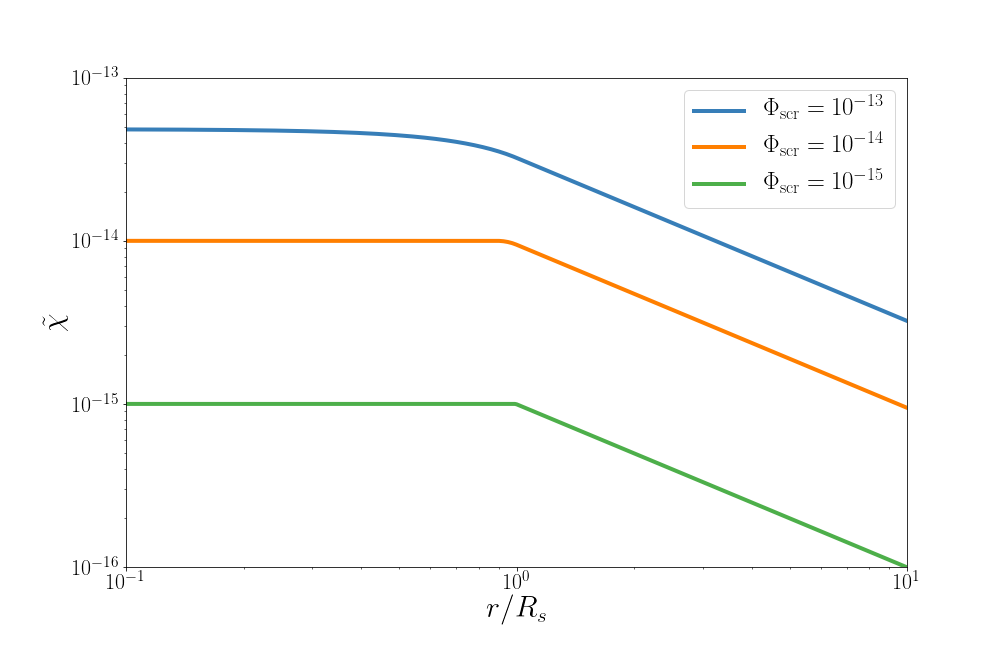
\includegraphics[width=1.0\linewidth]{{spherical_cham/starlike}.png}
% 	\caption{Chameleon profile for~several screening potentials. The~top solution is in~the~linear regime and~is identical to~the~gravitational potential. The~other two solutions are in~the~screened regime and~the~amplitude of~the~field is suppressed.}
% 	\label{fig:starlike}
% \end{figure}

% {\itshape
% Let us focus on~the~regime which cannot be treated analytical, i.e. regime between thin-shell and~thick-shell solutions. This regime corresponds to~the~situation when the~linear approximation (thick-shell) breaks down inside the~object, i.e. the~gravitational potential cancels screening potential somewhere inside the~object. We will denote $\Req$ the~\textit{equivalence radius} -- radius at~which the~Newtonian potential equals the~screening potential $|\Phi_G(\Req)|=\Phi_s$. By letting the~equivalence radius posses also negative values such as $(1+|\Req|/R_s)|\Phi_G(0)|=\Phi_s$ we can clearly distinguish between the~linear $(\Req<0)$ and~the~screening $(\Req>0)$ regime.}

% In~\autoref{fig:starlike_forces} we show the~behavior of~the~chameleon fifth force in~this regime. We see that for~the~linear regime the~fifth force is as strong as standard gravity (up to~the~factor $2\beta^2$). For~$\Req\ll R_s$ the~chameleon field manages to~catch up with~the~linear solution inside the~object and~there is no screening outside. As the~$\Req$ grows the~field is not able to~catch up with~the~linear solution while inside the~object and~the~force outside is screened.
% \begin{figure}
% 	\centering
% 	
\includegraphics[width=1.0\linewidth]{{spherical_cham/starlike_forces}.png}
% 	\caption{Chameleon force relative to~the~standard gravitational force for~several screening potentials (given through the~equivalence radius). For~$\Req\ll R_S$ there is no screening outside the~object. As the~$\Req$ grows the~chameleon enters the~screened regime.}
% 	\label{fig:starlike_forces}
% \end{figure}

\subsubsection{NFW Halo}
The~Navarro-Frenk-White (NFW) profile proposed by \textcite{1996ApJ...462..563N} describes the~distribution of~cold dark matter. The~NFW profile of~matter overdensity is given by
\eq{
	\label{NFW_rho}
	\delta\rho_{\rm NFW}(r)=\frac{\rho_c}{r/r_s\left(1+r/r_s\right)^2},
}
where $\rho_c$ is the~density scale and~$r_s$ is the~scale radius. We will also be using the~dimensionless radius $x\equiv r/r_s$. The~total mass of~the~halo is divergent (logarithmically) so we take a~cut-off at~the~radius $r_{200}$, which is defined as the~radius at~which the~density is 200 times the~critical density. Then the~mass of~the~halo is
\eq{
	M_{200}=\int_0^{r_{200}}4\pi r^2\rho(r)\dd r=4\pi\rho_cr_s^3\left(\ln(1+c)-\frac{c}{c+1}\right),
}
where $c\equiv r_{200}/r_s$ is the~concentration of~the~halo. For~a~given mass the~halo is fully characterized by the~concentration.

% For~NFW halo the~density is not constant as in~the~case of~compact spherical objects (stars). The~chameleon mass and~the~screened solution are therefore also not constant and~one does not have analytical solutions as in~the~case of~stars. However, for~realistic halo, the~density varies on~scales much larger than the~Compton wavelength of~the~chameleon. In~such cases, we can treat the~field as frozen in~the~same sense as in~the~case of~stars. Therefore we expect the~chameleon field to~behave in~a~similar way as in~the~case of~stars, i.e. to~follow the~Newtonian potential in~the~linear case and~to~have screened behavior for~more massive halos.

In~\autoref{fig:nfwlike_forces} we show the~chameleon fifth force. We see that the~behavior is indeed similar to~stars although the~field catches up much later. This is because there is no sudden drop in~density (and~mass of~the~field) where the~chameleon can start to~behave as free but rather the~mass is slowly dropping. This indicates that it will be much harder to~detect the~chameleon fifth force on~scales of~galaxies than for~star-like objects. This is of~course true only assuming the~screening potential is the~same on~all scales.
\begin{figure}
	\centering
	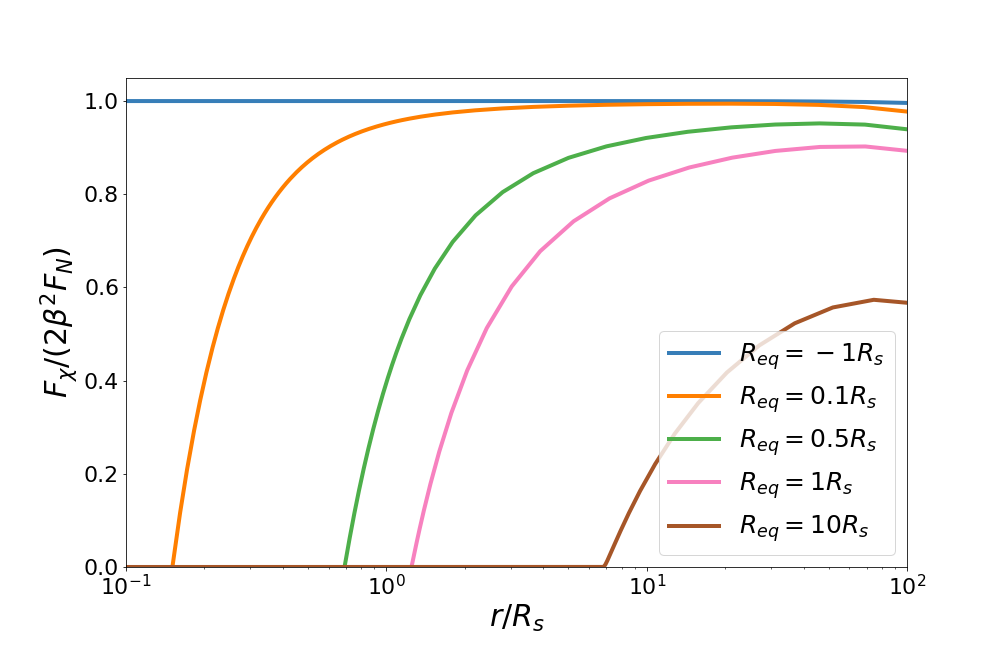
\includegraphics[width=1.0\linewidth]{{spherical_cham/nfwlike_forces}.png}
	\caption{Chameleon force relative to~the~standard gravitational force for~several screening potentials (given through the~equivalence radius). For~$\Req\ll R_S$ there is no screening outside the~object. As the~$\Req$ grows the~chameleon enters the~screened regime.}
	\label{fig:nfwlike_forces}
\end{figure}

The~meaning of~the~screening potential and~its connection to~the~Newtonian potential in~\eqref{eq:chi__scr_mean} is given by the~value of~the~field at~the~background, i.e. value that minimizes right side of~\eqref{eq:cham_u}. However, objects like stars or galaxy halos do not sit directly in~the~overall average density of~the~universe but rather in~galaxy halo or halo of~the~cluster of~galaxies. Therefore the~value of~the~effective screening potential is given by the~density of~the~background object we can consider as being in~infinity relative to~the~scale of~the~studied object. In~\autoref{fig:nfwlike_pot_eff} we show the~value of~this effective screening potential for~a~cluster of~galaxies of~a~typical size -- $M=10^{14} M_\odot, c=4$. We see that the~screening potential is greatly reduced in~inner parts of~the~galaxy cluster halo. For~this reason, we do not think it much likely to~observe the~effects of~the~chameleon field on~scales smaller than Mpc.

\begin{figure*}
	\centering
		\begin{subfigure}{1.0\linewidth}
			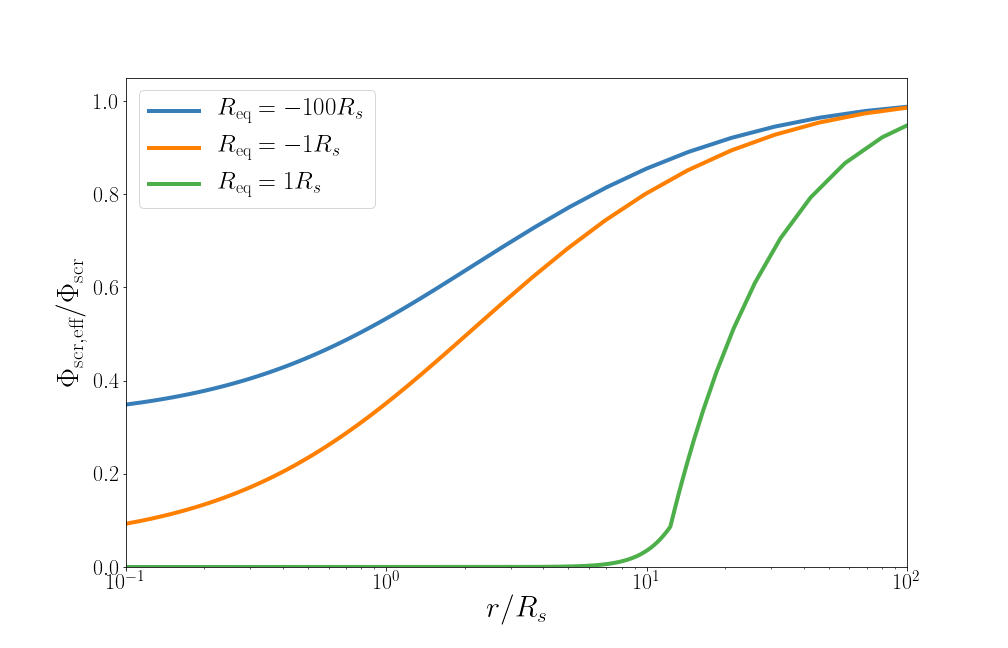
\includegraphics[width=1.0\linewidth]{{spherical_cham/nfwlike_pot_eff}.png}
		\end{subfigure}
		\begin{subfigure}{1.0\linewidth}
			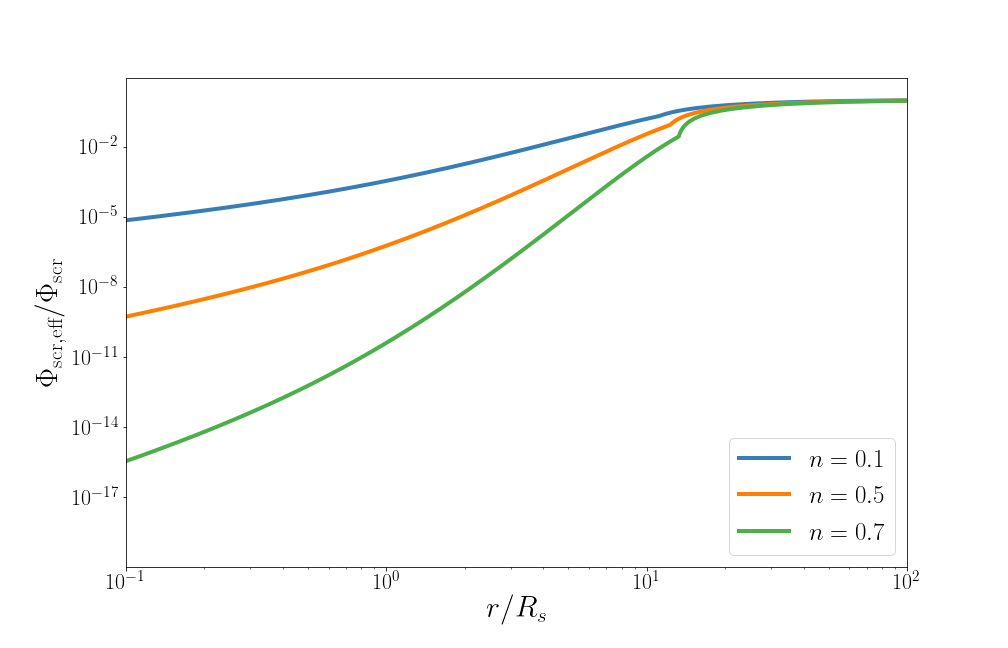
\includegraphics[width=1.0\linewidth]{{spherical_cham/nfwlike_pot_eff_n}.png}
		\end{subfigure}
		\caption{Effective screening potential relative to~the~screening potential for~a~cluster of~galaxies, $M=10^{14} M_\odot, c=4$. The~top Figure is shown for~several screening potentials (given through the~equivalence radius) while the~bottom for~different chameleon parameter $n$.}
		\label{fig:nfwlike_pot_eff}
\end{figure*}

As the~chameleon affects only non-relativistic matter it can be detected using a~combination of~dynamical measurements and~lensing measurements. Therefore, we considered what would be the~difference between the~mass distribution of~a~galaxy cluster measured via lensing (true mass) and~via dynamics of~enclosed galaxies. In~\autoref{fig:clustersYs} we plot this ratio for~five real clusters (simulated as having ideal NFW profile), see their parameters in~\autoref{tab:clusters}, and~for~four different values of~the~screening potential. We see that except for~the~case $\Phiscr=1$ one would need very precise (and~nowadays unrealistic) measurements of~the~mass distribution. We are therefore left with~only cosmological scales of~tens of~Mpc and~larger to~study the~chameleon. We will study this case in~\autoref{chpt:app_sims}.
\begin{table}[hbt]
	\centering
	\begin{tabular}{lcc|lcc}
		\hline \hline
		Cluster & $c$ & $M$ & Cluster & $c$ & $M$ \\
		\hline
		ClG 0054-27 & $1.2$ & $0.42\cdot10^{14}$ &
		Cl 0016+1609 & $2.1$ & $1.12\cdot10^{14}$ \\
		MS 2137.3-2353 & $13$ & $2.9\cdot10^{14}$ &
		ClG 2244-02 & $4.3$ & $4.5\cdot10^{14}$ \\
		MS 0451.6-0305 & $5.5$ & $18\cdot10^{14}$ & & & \\
		\hline \hline
	\end{tabular}
	\caption{Properties of~clusters simulated as perfect NFW halos: concentration $c$ and~mass $M [M_\odot]$. Parameters are taken from \textcite{2007MNRAS.379..190C}}
	\label{tab:clusters}
\end{table}

\begin{figure*}[!hbt]
\begin{adjustwidth}{-1cm}{-1cm}
	\centering
		\begin{subfigure}{0.5\linewidth}
			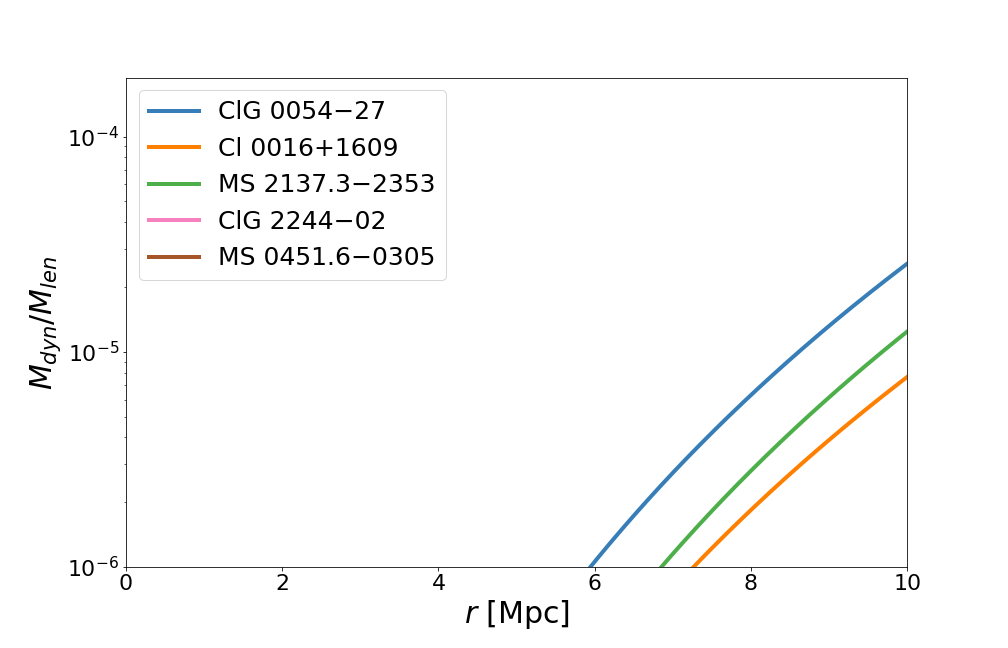
\includegraphics[width=1.0\linewidth]{{spherical_cham/clustersYs_-6}.png}
			\caption{$\Phiscr=10^{-6}$}
		\end{subfigure}%
		\begin{subfigure}{0.5\linewidth}
			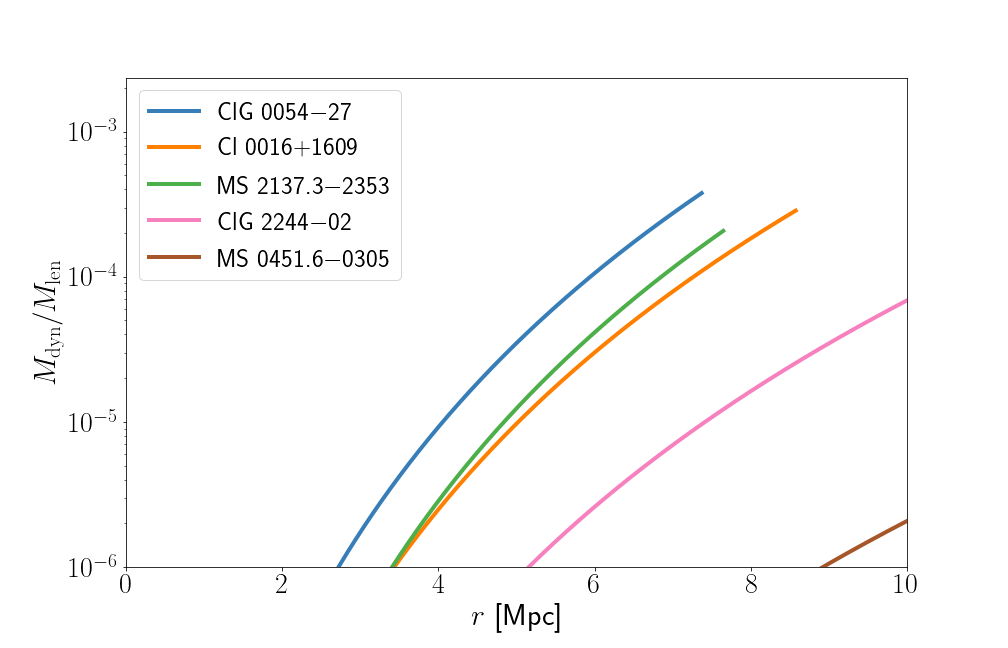
\includegraphics[width=1.0\linewidth]{{spherical_cham/clustersYs_-4}.png}
			\caption{$\Phiscr=10^{-4}$}
		\end{subfigure}
		\begin{subfigure}{0.5\linewidth}
			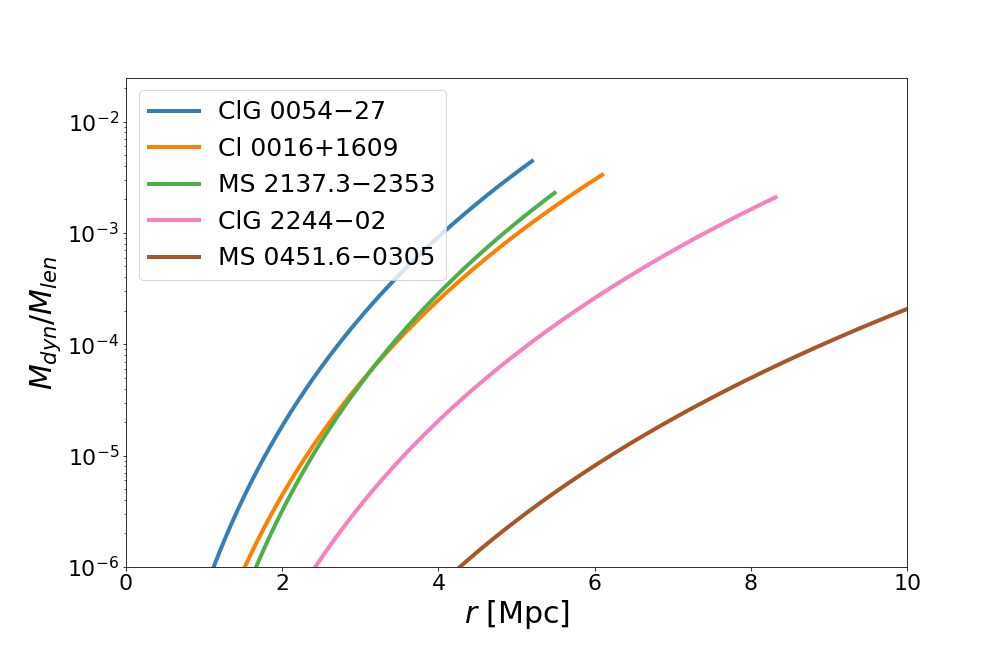
\includegraphics[width=1.0\linewidth]{{spherical_cham/clustersYs_-2}.png}
			\caption{$\Phiscr=10^{-2}$}
		\end{subfigure}%
		\begin{subfigure}{0.5\linewidth}
			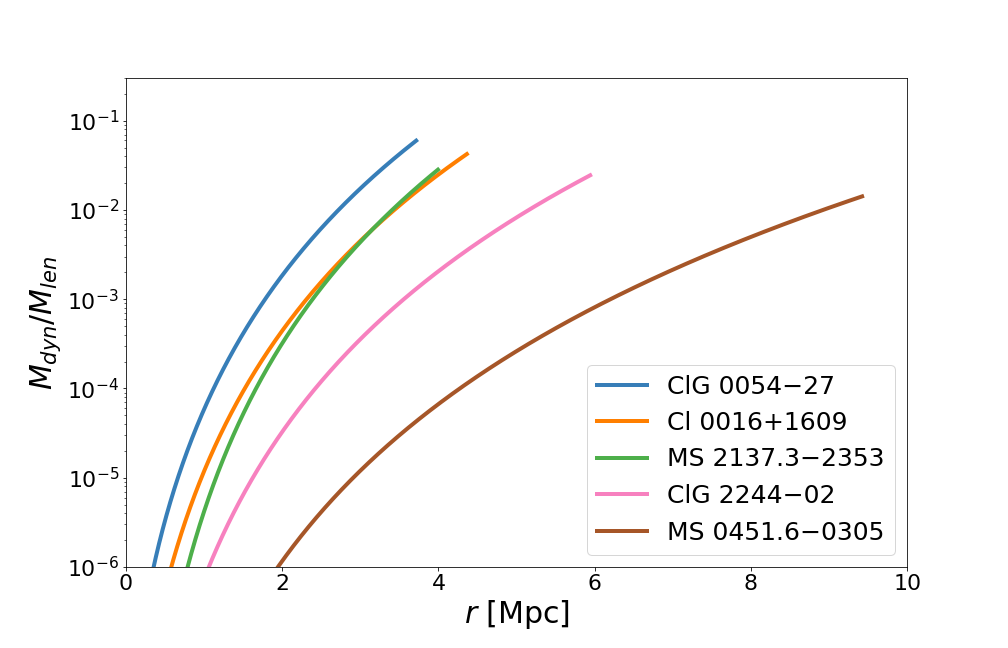
\includegraphics[width=1.0\linewidth]{{spherical_cham/clustersYs_0}.png}
			\caption{$\Phiscr=10^{0}$}
		\end{subfigure}
	\end{adjustwidth}
		\caption{Effective dynamical mass of~the~clusters relative to~the~actual (lensing) mass of~the~cluster. Cluster properties are shown in~\autoref{tab:clusters}.}
		\label{fig:clustersYs}
\end{figure*}

%%%%%%%%%%%%%%%%%%%%%%%%%%%%
% Other theories
%%%%%%%%%%%%%%%%%%%%%%%%%%%%
\section{Other theories}
In this section we briefly mention some of the other theories od modified gravity. This list is in no way complete and serves only as an example of different approaches to modifications of gravity. See references for further reading.
\subsection{Quintessence}
Quintessence, from the Latin ``fifth element'', is according to ancient and medieval philosophy the fifth element, or ether, supposed to be the constituent matter of the heavenly bodies after air, fire, earth, and water. The name quintessence, or the $Q$ component, was first used by \textcite{1998PhRvL..80.1582C} for the canonical scalar field $\phi$ evolving along a potential $V(\phi)$. Such a dynamical field can reproduce the late-time acceleration with the equation of state $w=w(t)\approx1$. Although quintessence can alleviate the coincidence problem of dark energy via the so-called tracker solution, it still suffers by the fine-tunning problem as the potential needs to be flat enough to lead to the slow-roll inflation today with an energy scale $\rho_{DE}\simeq10^{-120}\Mpl^4$ and a mass scale $m_\phi\lesssim10^{-33}$ eV. However, such fine-tuned potentials can be constructed within the framework of particle physics.

Quintessence is one of the simple models of dark energy as it is a canonical scalar field that interacts with all the other components only through standard gravity. The Lagrangian density for the quintessence field is
\eq{
\label{Qlagr}
\LL_\phi=-\frac12(\partial\phi)^2-V(\phi)
}
We can compute the stress-energy tensor as
\eq{
T^\phi_\uv\equiv\frac{-2}{\dg}\frac{\delta(\dg\LL_\phi)}{\delta g^\uv}=\partial_\mu\phi\partial_\nu\phi-g^\uv\left(\frac12(\partial\phi)^2+V(\phi)\right).
}
Now, the energy density and pressure are given by components of the stress-energy tensor. For FLRW background and $\phi$ only time-dependent we get
\eq{
\rho_\phi=-T^0_0=\frac{1}{2}\dot{\phi}^2+V(\phi)\ \ \ \ p_\phi=\frac{1}{3}T^i_i=\frac{1}{2}\dot{\phi}^2-V(\phi).
}
Equation of state for the quintessence is then
\eq{
\label{eosQ}
w\equiv\frac{p}{\rho}=\frac{\dot{\phi}^2-2V(\phi)}{\dot{\phi}^2+2V(\phi)}\,.
}
We require the condition $w<-1/3$ to realize the late-time cosmic acceleration, which translates into the condition  $\dot{\phi}^2<V(\phi)$, i.e. the potential needs to be shallow enough for the field to evolve slowly along the potential. For a slow-rolling field such as $\dot{\phi}\ll V(\phi)$ equation of state \eqref{eosQ} reduce to $w\approx-1$ as indicated by cosmological measurements.

The variation of \eqref{Qlagr} with respect to $\phi$ gives us the equation of motion for the scalar field $\phi$
\eq{
\ddot{\phi}+3H\dot{\phi}^2+V_{,\phi}=0\,.
}

Depending on which term and when determines the evolution of the field, the quintessence models have been dynamically classified into \textit{freezing} models and \textit{thawing} models \parencite{2005PhRvL..95n1301C}. In the freezing models the field was rolling along the potential in the past, but the movement gradually slows down as the field approaches the minimum of the potential $(\dot{\phi}\rightarrow0)$ and the system enters the phase of the cosmic acceleration $(w\rightarrow-1)$. In the thawing models, the field was initially frozen $(\dot{\phi}\approx0)$ in the early matter era because of the Hubble friction (the term $H\dot{\phi}$) until recently and then it begins to evolve once $H$ drops below $m_\phi$ and $w$ evolves from $-1$.

A potential of the freezing models is for example
\eq{
\label{Qtr}
V(\phi)=M^{4+n}\phi^{-n}\ (n>0),
}
which appears in the fermion condensate model as dynamical supersymmetry breaking \parencite{1999PhRvD..60f3502B}. This potential does not possess a minimum and hence the field rolls down the potential toward infinity. Another example of potential in the freezing models is
\eq{
V(\phi)=M^{4+n}\phi^{-n}\exp{(\alpha\phi^2/\Mpl^2)},
}
which can be constructed in the framework of supergravity \parencite{1999PhLB..468...40B}. This potential has a minimum at which the field is eventually trapped (corresponding to $\dot{\phi}=0$ and hence $w=-1$).

The broader class of potentials belonging to the thawing models are so-called hilltop quintessence models \parencite{2008PhRvD..78l3525D}, in which the scalar field is rolling near a local \textbf{maximum} in the potential but it begins to roll down around the present. A particular example that is well-described by this model is the pseudo-Nambu-Goldstone Boson (PNGB) model of \textcite{1995PhRvL..75.2077F}, for which the potential is given by
\eq{
V(\phi)=M^{4}\left[\cos{(\phi/f)}+1\right].
}
\subsection{K-essence}
Quintessence models are based on a scalar field with a canonical kinetic term and a slowly varying potential. However, in the context of particle physics there appear scalar fields with non-canonical kinetic terms. In \textcite{1999PhLB..458..209A} it is shown that a large class of scalar fields with non-canonical kinetic terms can, without the help of potential terms, drive an inflationary evolution starting from rather generic initial conditions. The Lagrangian density for the k-essence is
\eq{
\label{Klagr}
\LL_K=P(\phi, X),
}
where $X=-\frac12(\partial\phi)^2$ is the canonical kinetic energy and the function $P(\phi, X)$ must vanish for $X\rightarrow0$ (otherwise there would be some potential term). 

The energy-momentum tensor of the k-essence is given by
\eq{
T^K_\uv\equiv\frac{-2}{\dg}\frac{\delta(\dg\LL_K)}{\delta g^\uv}=P_{,X}\partial_\mu\phi\partial_\nu\phi+g^\uv P,
}
which is of the form of a perfect fluid, $T_\uv=(\rho+p)u_\mu u_\nu+g_\uv p$, with a four-velocity $u_\mu=\partial_\mu\phi/\sqrt{2X}$, pressure $p_K=P$ and energy density
\eq{
\rho_K=2XP_{,X}-P.
}
The equation of state of the k-essence is then
\eq{
w_K=\frac{p_K}{\rho_K}=\frac{P}{2XP_{,X}-P},
}
which is $w_K\approx-1$, as long as the condition $XP_{,X}\ll P$ is satisfied.

In the low-energy effective string theory appear higher-order derivative terms coming from $\alpha$ and loop corrections to the tree-level action \parencite{2003PhR...373....1G}. The k-essence action for these theories is for example
\eq{
P=K(\phi)X+L(\phi)X^2.
}
Phantom or ghost scalar fields with a negative kinetic energy $-X$ and $w\lesssim-1$ can also fit the current observations. These ghost fields generally suffer from a quantum instability problem unless higher-order terms in $X$ or $\phi$ are taken into account in the Lagrangian density \parencite{2010deto.book.....A}. The action of the so-called dilatonic ghost condensate model is \parencite{2004JCAP...07..004P}
\eq{
P=-X+e^{\kappa\lambda\phi}X^2/M^4.
}
\subsection{Gauss-Bonnet Dark Energy Models}
In \fR\ gravity one adds the general function of the Ricci scalar. But in principle, one can add general functions of the Ricci and Riemann tensors as well, e.g. $f(R,R_\uv R^\uv,R_{\alpha\beta\gamma\delta}R^{\alpha\beta\gamma\delta},...)$ \parencite{2005PhRvD..71f3513C}. These Lagrangians are generally plagued by the existence of ghosts.  However, there exists a combination of Ricci and Riemann tensors that keeps the equations at second-order in the metric and does not necessarily give rise to instabilities -- so-called Gauss-Bonnet term $\GB$ coupled to a scalar field
\eq{
\GB\equiv R^2-4R_\uv R^\uv+R_{\alpha\beta\gamma\delta}R^{\alpha\beta\gamma\delta}.
}
The Gauss-Bonnet term is the unique invariant for which the highest (second) derivative occurs linearly in the equations of motion and thus ensuring the uniqueness of solutions. The Gauss-Bonnet term naturally arises as a correction to the tree-level action of low-energy effective string theories \parencite{2000PhR...337..343L}. The starting action is given by
\eq{
S=\int\dd^4x\dg\left[\frac{\Mpl^2}{2}R-\frac{\gamma}{2}\left(\nabla\phi\right)^2-V(\phi)+f(\phi)\GB\right],
}
where $\gamma=\pm1$ (+1 for the canonical scalar). For more details see \textcite{2005PhRvD..71l3509N,2006JCAP...06..004N,2013PhRvD..87h4037C}.
\subsection{Braneworld Models}
In the braneworld model of Dvali, Gabadadze, and Porrati \parencite[DGP model][]{2000PhLB..485..208D} the 3-brane is embedded in a Minkowski bulk spacetime with infinitely large extra dimensions. The theory gives rise to the correct 4D potential at short distances whereas at large distances the potential is that of a 5D theory. The action of the theory is
\eq{
S=\frac{M^3_{(5)}}{2}\int\dd^5X\dgt\tR+\frac{\Mpl^2}{2}\int\dd^4x\dg R + \int\dd^4x\dg \LL_m,
}
where $g_{AB}(X)=g_{AB}(x,y)$ denotes a 5D metric for which the 5D Ricci scalar is $\tR$ and $M_{(5)}$ is the 5D Planck mass. Capital letters are used for 5D quantities $(A,B=0,1,2,3,5)$. The brane is located at $y=0$. The induces 4D metric on the brane is denoted by
\eq{
g_\uv(x)\equiv\tilde{g}_\uv(x,y=0).
}
The cross-over scale $r_0$ is defined by
\eq{
r_0\equiv\frac{\Mpl^2}{2M^3_{(5)}}.
}
At short distances $r\ll r_0$ gravity behaves as usual 4D theory, i.e the gravitational potential has correct $1/r$ behavior (except small logarithmic repulsion term). On the other hand at large distances $r\gg r_0$ the potential scales as $1/r^2$ according to the laws of 5D theory.

The presence of the extra dimension has severe consequences on the cosmology as well. It can be shown \parencite{2010deto.book.....A,2009PhLB..674..237M} that the matter-dominated Universe approaches the de Sitter solution $H=r_0\mins$. This cosmological solution drives our Universe into the self-inflationary regime without dark energy. From $H_0\approx r_0\mins$ we get $M_{(5)}\approx10-100$ MeV.
\subsection{Massive Gravity}
The idea to give a mass to the graviton (infrared modification of gravity) is not new and has been investigated since the first years of General Relativity. It is a less minimal theory than \fR\ theories or modified gravities with an extra scalar field because it introduces three new degrees of freedom rather than one. By giving a mass $m$ to the graviton we deform the classical potential to the Yukawa profile $\sim\frac1r e^{-mr}$ which departs from the classical one at distances $r>1/m$. By choosing the graviton mass to be of the order of the Hubble constant $m\sim H$ one can hope to explain the acceleration of the universe without dark energy.

The simplest theory for a non-self-interacting massive graviton is the Fierz-Pauli theory of \textcite{1939RSPSA.173..211F}. The action for a single massive spin 2 particle in flat space, carried by a symmetric tensor field $h_\uv$ is
\eq{
\begin{split}
S=&\int\dd^4x\Big[-\frac12\partial_\lambda h_\uv\partial^\lambda h^\uv+\partial_\mu h_{\nu\lambda}\partial^\nu h^{\mu\lambda}-\partial_\mu h^\uv\partial_\nu h \\
&+\frac12\partial_\lambda h \partial^\lambda h-\frac12 m^2\left(h_\uv h^\uv-h^2\right)\Big]+S_m.
\end{split}
}
Any other combination of $h_\uv h^\uv$ and $h^2$ would lead to instabilities. Varying the action with respect to $h_\uv$ yields the equation of motion
\eq{
R_\uv-\frac12Rg_\uv+\frac12m^2(h_\uv-h\eta_\uv)=\frac{1}{\Mpl^2}T_\uv,
}
where all quantities are linearized around $\eta_\uv$.

Because of the so-called vDVZ discontinuity (``van Dam-Veltman-Zakharov'') in the propagator of a graviton, the Fierz-Pauli theory leads to different physical predictions from those of GR regardless the mass of the graviton (even when $m\to0$). The Vainshtein mechanism \parencite{1972PhLB...39..393V} allows in principle to get rid of the vDVZ discontinuity by introducing non-linear Fierz-Pauli gravity.

The Vainshtein mechanism is another example of the screening mechanism and restores the continuity with GR on scales below the so-called Vainshtein radius $r_V$, defined as
\eq{
r_V\equiv(GM/m^4)^{1/5}.
}
Much below the Vainshtein radius, which grows as the graviton's mass approaches $0$, only linear terms play a crucial role and the GR is restored.

For more about the massive gravity and the Vainshtein mechanism see e.g. \textcite{2013CQGra..30r4001B,2012RvMP...84..671H}.

\subsection{Acceleration without Dark Energy}
So far we studied some kind of dark energy -- either in the form of an exotic matter or by modifying gravity itself. But this need for dark energy as an explanation of the acceleration comes from our observations which are based on the presumption of the homogeneous and isotropic Universe. What we observe are different expansion rates at different distances rather than an increase in the expansion rate at all distances. But this can be caused by strong inhomogeneities in the distribution of matter rather than by an accelerating Universe.
\subsubsection{Void models}
The basic idea behind void models is that we live in the middle of a huge spherical region which is expanding faster because it is emptier than the outside. That means that the Universe as a whole does not accelerate but that we observe an \textit{apparent} cosmic acceleration. The edge of this void should be located around $z\sim0.3-0.5$, the value at which in the standard interpretation we observe the beginning of the acceleration. These models are described by the Lema\^\i tre-Tolman-Bondi (LTB) spherically symmetric metric -- the generalization of a FLRW metric in which the expansion factor along the radial coordinate is different relative to the surface line element $\dd\Omega^2$ \parencite{2013JCAP...02..047D,2006PhRvD..73h3519A}.

The inhomogeneous LTB model matches to the supernovae data and the location of the first acoustic peak of the CMB temperature power spectrum but cannot satisfactorily reproduce the entire CMB angular power spectrum \parencite{2011JCAP...02..013C}. The observed isotropy of the CMB radiation implies that we must live close to the center of the void -- nearer than 15 Mpc \parencite{2006PhRvD..74j3520A}. Moreover, there is no valid mechanism at present to explain the formation of such huge inhomogeneities, let alone one with our Galaxy near the center.
\subsubsection{Backreaction}
Unlike the void models, which regard the acceleration as an apparent one, \textit{backreaction} models try to explain the cosmic acceleration by arranging inhomogeneities so that the deviation from the FLRW metric can produce a real acceleration \parencite{2011CQGra..28w5002S,2004JCAP...02..003R,2005PhRvD..72b3507M}. Because GR equations are non-linear, averaging the inhomogeneities and then solving the GR equations (which is the usual approach) is not the same as first solving the full (inhomogeneous) GR equations and then averaging them -- the expected value of a non-linear function is not the same as the non-linear function of the expected value.

Any large inhomogeneities must be concealed from our sight to fit observations. Strong peculiar velocities instead of strong density fluctuations can do this job, but there are strong constraints on peculiar velocities from e.g., the kinematic Sunyaev--Zel'dovich effect. Moreover, the accompanying anisotropy is another source of observable effects difficult to accommodate with current observations.

\section{Parametrization of models}
We saw in the previous chapter that at the background level the evolution is governed by Friedman equations \eqref{eq:Friedmann} -- \eqref{eq:Friedmann-continuity} and consequently omega parameters \eqref{eq:omega} and Hubble parameter $H$ which can be obtained, e.g., from distance measurements. As we discussed, the cosmological constant is not the only possible explanation of the accelerated expansion and the equation of state \(w\) of dark energy does not have to be exactly \(w=-1\). For the arbitrary equation of state $w_{DE}=p_{DE}/\rho_{DE}$ in the flat Universe with a negligible contribution of radiation we can obtain the following equation
\eq{
    \label{eq:w_de}
    w_{DE}(z)=\frac{(1+z)(E^2(z))'-3E^2(z)}
                   {3\left[E^2(z)-\Omega_{m,0}(1+z^3)\right]}\,,
}
where a prime denotes derivative with respect to \(z\). We see that \(w_{DE}\) cannot be determined solely from \(E(z)\) (obtainable through distance measurements) and we need also present density of matter \(\Omega_{m,0}\). However, if we parametrize \(w_{DE}\) in some way as it is usually done through measurements of \(E(z)\) at several redshifts we can constraint both \(w_{DE}\) and \(\Omega_{m,0}\).

Several parametrization  of \(w_{DE}\) have been proposed so far. We can write such parametrization  in the form
\eq{
    w_{DE}=\sum_{n=0}w_nx_n(z)\,,
}
where he expansions can be given by
\eq{
    & \rm{(i) Redshift:}      & x_n(z) &= z^n\,, \\
    & \rm{(ii) Scale factor:} & x_n(z) &= (1-a)^n=\left(\frac{z}{1+z}\right)\,, \\
    & \rm{(iii) Logarithmic:} & x_n(z) &= \left[\ln\left(1+z\right)\right]^n\,.
}
Parametrization (ii) is usually written for \(n\leq1\) as \(w=w_0+w_a(1-a)\).

For the generic \fR\ gravity, the equation of state is given by \parencite{2013qopu.conf...73B}
\eq{
    w_{DE} = \frac{-(1/2)(F\R R-F)+\ddot F\R+2H\dot F\R-(1-F\R)\left(2\dot H + 3H^2\right) }
                  {(1/2)(F\R - F) - 3H\dot F\R + 3 (1-F\R)H^2}\,,
}
which then can be compared with observations \eqref{eq:w_de}. For different examples of evolution of $w_{DE}$ see, e.g., \textcite{2020arXiv200707717A}.